\def \hmina {\hspace{-0.1in}}
\def \hminb {\hspace{-0.2in}}

\def \fgw {2in}
\def \fgh {1in}

% \begin{floatingfigure}[r]{2in}  (and \end{..})

\begin{figure}[t]
    \centerline{
        % \hmina
        % {\input{data/eval-ms}}
        % \hminb
        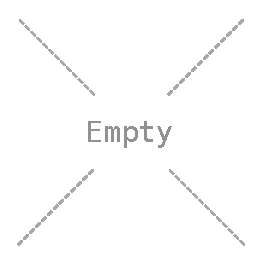
\includegraphics[height=\fgh]{empty.eps}
    }

    \mycaption{fig:eval-ms}{Mirrored and Selective I/O performance}{Median
    sequential and random I/O compared to baseline. Each cluster of 3 dots
    between configurations represents the 7:3, 5:5, and 3:7 ratios as discussed
    in \cref{subsec:eval-dynamic}.}
\end{figure}
